%%%%%%%%%%%%%%%%%%%%%%%%%%%%%%%%%%%
%% Starting Appendix at a new page, 
%% Resetting section counters
%%%%%%%%%%%%%%%%%%%%%%%%%%%%%%%%%%%
\clearpage 
%\newpage
\setcounter{section}{0}

\section*{\huge{\textsc{Appendix}}}
\label{sec:appendix}

%Extra experiments/analysis consists of the following:
%\begin{itemize}
%    \item Impact of different kinds of lens -- wall mount vs ceiling mount
%    \item Gradual build of dust leading to missed detection
%showing time domain analysis not enough
%    \item \cout-based definition of degree of failure
%    \item lens-based failures deployed in MSR cafeteria
%	\item Frequently Asked Questions (FAQs)
%    \item Implementation details such as preprocessing, analysis and interpretation of hardware signals.
%    \item Additional experiments and observations from real-world deployments and in-lab studies,
%\end{itemize}

%\section{\sol}
%
%\subsection{Goals and Target Audience}
%\quad \underline{\bfseries Detect failures:} Sensors can give faulty data due to the incorrect operation of various physical components involved in the sensing process. We seek to detect and isolate such failed sensors. %data that is not a faithful representation of the physical phenomenon.
%
%\underline{\bfseries Diagnose failures:} In addition to detecting failures, we perform failure diagnosis to identify the cause of the failure. We use domain-knowledge of the sensing physics and understanding of how different failures can impact the physics. This aids in repair and performing quality-control checks.
%
%\underline{\bfseries Edge-based solution:} Our solution is tailored for edge platforms (Raspberry Pi, Arduino Microcontrollers) that are interfaced directly to multiple sensors via GPIO. %\st{Being low-cost, these sensors have low compute or storage capabilities.}
%Edge-based reliability solutions allows us to reject data from faulty sensors in IoT deployments thus saving the cost of both \ca the edge to cloud network bandwidth and \cb cloud compute consumed by faulty data.
%
%\underline{\bfseries Target Audience:} Our solution benefits two sections of the community: \ca engineers developing and deploying IoT/Edge computing for occupancy sensors (\eg Smart Buildings), \cb manufacturers of occupancy sensors can use the insights from this work for their sensor hardware designs.

\section{Frequently Asked Questions (FAQs)}
\label{sec:app}
%\begin{wrapfigure}{L}{0.5\textwidth}
%	\begin{minipage}{0.5\textwidth}
%		\centering
%		\includegraphics[width=\textwidth]{figures/pir/commercial_aout/IMG_20190813_170956.jpg}
%		\caption{\textsc{\aout} from a commercial-grade PIR sensor showing a waveform similar in nature to the low-cost PIR sensor. Note that we had to rework the sensor to extract the \aout signal from the board.}
%		\label{fig:aout_commercial}
%	\end{minipage}
%
%\end{wrapfigure}


\begin{description}[style=nextline]
	\item[Q: Where does \sol \textit{detect and diagnose} faults? ] A: \sol performs detection and diagnosis on collected data at the edge device, and does not need any additional hardware. Edge devices are commonly present in sensor deployments and are responsible to aggregate data from multiple sensors and transmit it to the cloud. We use the edge to execute \sol.
	\item[Q: Does \sol require \textit{cloud connectivity}?] 
	A: \sol performs all the computation on the edge and does not require cloud connectivity. As it detects failures on the edge and rejects incorrect data, this saves cloud-edge network bandwidth as well as ensures data from broken sensors do not reach the cloud, thereby enabling better data analytics at the cloud as well. 
	\item[Q: Does \sol detect faults at runtime? Is it instantaneous?]
	A: \sol is used to detect failures by analyzing samples over a window of 256 -- 1024 samples \ie 5 -- 20 seconds at a sampling rate of 50 Hz. Thus, it can be used to detect anomalies at runtime. In addition, \sol is non-intrusive and does not involve disassembling or uninstalling the sensor. However, the typical use case is a post-analysis \eg once in a day to find out failing sensors since edge devices are typically resource constrained.
	\item[Q: Does \sol require special sensors?]
	A: \sol requires a PIR sensor that exposes the \aout signal \ie output of pyroelectric element. Currently, not all PIR sensor manufacturers expose \aout signal in their sensor. Note however that \textit{every} PIR sensor contains the \aout signal, as it is a core part of the pyroelectric element physics. 
	\item[Q: What can PIR sensor manufacturers takeaway from \sol?]
	A: We use this work to make sensor manufacturers include the signal \aout in all their sensor designs as it would enable fault detection and diagnosis at the edge.
	\item[Q: Are the failures artificial?]
	A: It is a criticism that \sol handles only artificially-induced failures. However, this is not true. The failures induced are those observed by IoT/Smart Building technicians and engineers who deploy sensors in our buildings in US and India. We recreate these failures on cheap sensors as it is not feasible to perform large-scale deployment with expensive sensors typically seen in modern buildings.
	%\item[Q: What challenges did you encounter?]
	%A: Since the data collected was of occupancy, we had to pause the work during the peak lockdown times (April to August 2020) of the pandemic and slowly resumed only once the lockdown had eased.
	\item[Q: Does \sol work with high-grade PIR sensors?]
	A:  While our work focused on low-cost, commodity, large-scale, cheap deployments of PIR sensors, the physics of sensing is identical in commercial-grade PIR sensors as well. We accessed a PIR sensor from our building ceiling and analyzed the \aout waveform by connecting it to an oscilloscope. In our preliminary observations, we saw that the shape of \aout is similar to that we saw in low-cost sensors. %The waveform of \aout observed from our sensor is shown as a oscilloscope snapshot in {\bfseries Fig.~\ref{fig:aout_commercial}}. 
	This similarity in the nature of \aout waveforms show promise to that our analysis and techniques can be extended to commercial-grade PIR sensors as well. As each of these sensors cost around \$200, we could not study conduct a study on different failures due to their exorbitant cost.
\end{description}

%\section{Implementation Details} %We cover the impact of changing window size on the accuracy of detection of faults. 
%We know from ~\cite{an_murata} that pyroelectric sensors have a cut off frequency of 10 Hz. Therefore, we analyze the frequency distribution within this range. This requires that we collect sensor samples at a frequency greater than Nyquist rate ($f_N$) \viz $\ge$ 20 Hz ( \ie inter-sample duration $\le$ 50 ms).

%The hardware signals we use for failure detection are - \ca Final output of the sensor \viz \cout and \cb Intermediate output at the pyroelectric element \viz \aout. Recall that our hypothesis being that \aout, accompanied by computationally low-cost processing and analysis, can be used for detecting fault detection and diagnosis.

%\subsection{Windowing} To enable computationally efficient analysis of $A_{out}$, we partition the signal in the time domain - each such partition is termed a window. This techique, common in signal processing applications, allows us to perform fault detection in a piecemeal manner. The size of each of these partitions is decided by the application - in our case we vary the window in the range between 5 seconds to 20 seconds. This is so choosen since this is typically the duration for crossing in front of the detection region of a PIR sensor.

%\subsection{Cost Analysis of PIR sensors in our building} \label{subsec:cost} Each PIR sensor in our building is priced at \$300 with it being refreshed every 10 years. Our building has 4 floors each comprising 61 rooms and 6 aisle areas giving a total of 244 rooms and 24 aisle areas. As a result, there are more than 300 occupancy sensors, giving a total recurring cost of \$90000 every 10 years, which is expensive.

%\subsection{Analysis of High-grade PIR Sensors}


%\subsection{Different types of lens} Another factor that determines the nature of the \aout curve is the nature of the lens used on the PIR sensor. Typically, an inline lens is used for the wall-mount version and a round lens is used for the ceiling-mount version. We used a wall-mount PIR sensor in our experiments though our analysis is equally applicable to ceiling-mount sensors.

%ashish
%Move to main
% \begin{figure}[ht]
% 	\centering
% 	\begin{subfigure}[t]{0.48\textwidth}
% 		\centering
% 		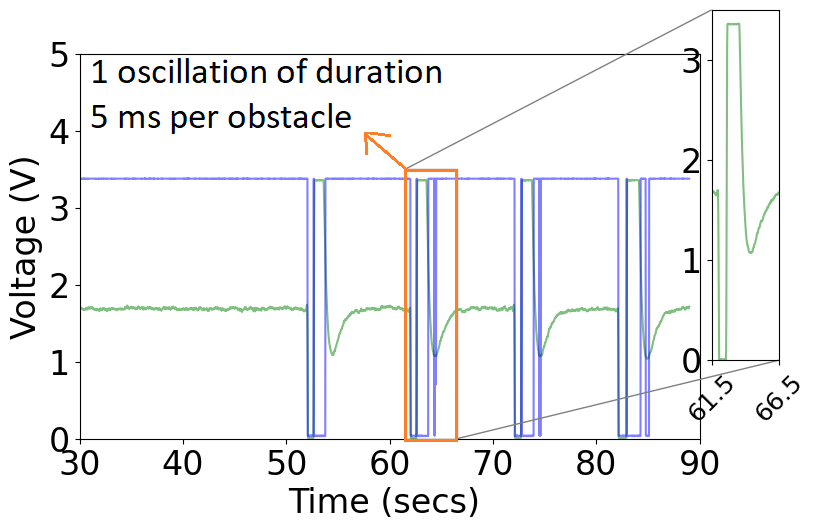
\includegraphics[width=\textwidth]{figures/lens_types/inline_lens.png}
% 		\caption{Inline lens (wall-mount)}
% 		\label{fig:inline_lens}
% 	\end{subfigure}	
%     \hspace{1ex}
% 	\begin{subfigure}[t]{0.48\textwidth}
% 		\centering
% 		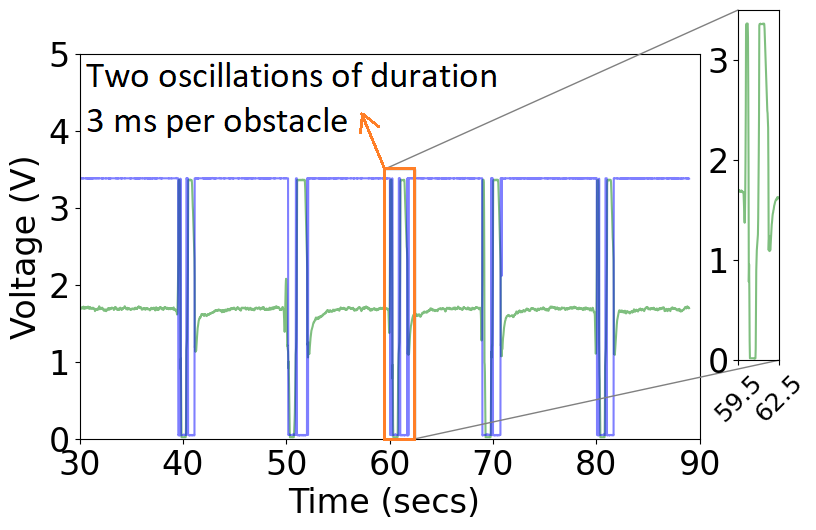
\includegraphics[width=\textwidth]{figures/lens_types/round_lens.png}
% 		\caption{Round lens (ceiling-mount)}
% 		\label{fig:round_lens}
% 	\end{subfigure}	   
% 	\caption{Effect of different types of lens on the \aout curve -- the inline lens type produces a single curve whereas a round lens type produces two curves per obstacle.}
% 	\label{fig:pir_sensor_different_lens}
% \end{figure}

%\textbf{Summary (Figure~\ref{fig:pir_sensor_different_lens})} shows the variations in \aout between the two types of lens -- \ca Inline lens has a wider curve compared to round lens and \cb Ceiling lens has double number of oscillations of \aout curve per obstacle.

%moved to main
%\subsection{Variability in Fault Classes} %In \S\ref{subsec:controlled}, we observed that the impact of failures in PIR sensors, from classes I through V cause certain effects on nature of \aout and \cout. While we developed a structural taxonomy in \S\ref{subsec:taxonomy}, 

%We note that failures need not be binary in nature. There can be partial failures. Consequently, there are variations in each of the failure classes. %that can lead to slight deviations in the failure modalities. 
%For example, in Class I faults, we observe that the amount of variance of \aout depends on the extent of dislodging of the lens cap from the sensor board. Similarly, Class II faults have different signatures depending on the whether the damage is a puncture or deformation. In this section, we describe some of the variations in Class III faults. 
%As with the taxonomy, our focus is on the practical, common and most frequently occurring failures seen in discussion with Building IoT engineers.
% ashish

%\begin{figure*}[htbp]
%	\centering
%	%\vspace{-1\baselineskip}
%	\begin{subfigure}[t]{0.23\textwidth}
%		\centering
%		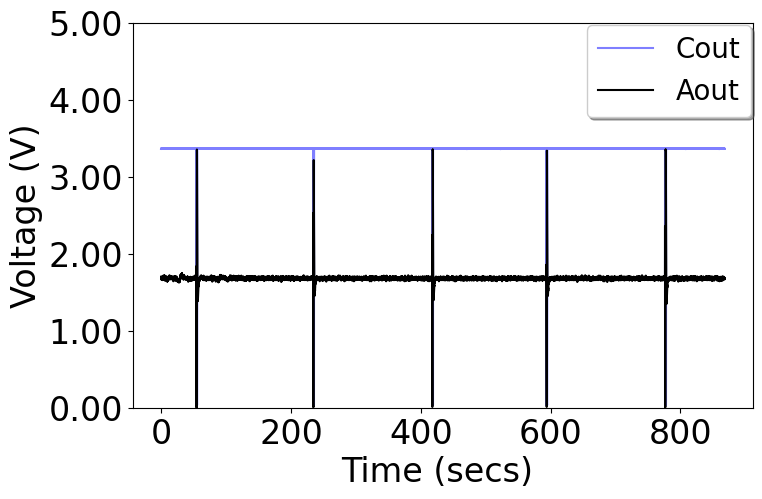
\includegraphics[width=\textwidth]{figures/gradual_degradation_dust/Stage0.png}
%		\caption{Clean Sensor : Working}
%		\label{fig:pir_sensor_classIII_fault_good_moved}
%	\end{subfigure}
%	\hspace{1ex}
%	\begin{subfigure}[t]{0.23\textwidth}
%		\centering
%		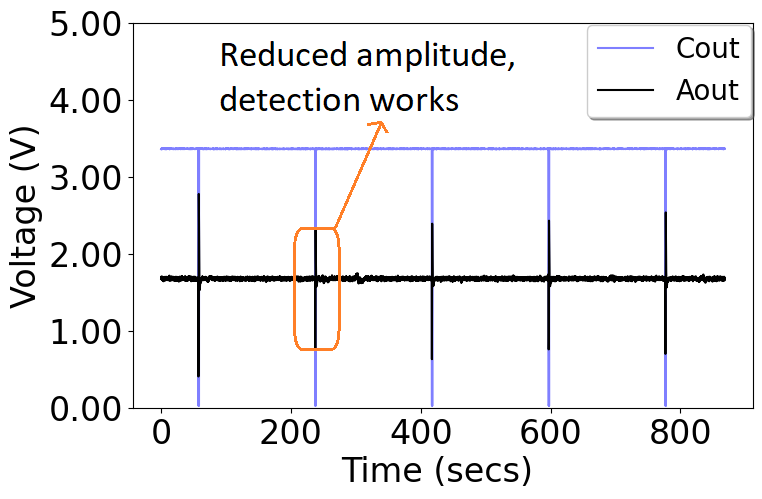
\includegraphics[width=\textwidth]{figures/gradual_degradation_dust/Stage1.png}
%		\caption{Degraded Sensor : Still Working}
%		\label{fig:pir_sensor_classIII_fault_bad1_moved}
%	\end{subfigure}	
%	\hspace{1ex}
%	\begin{subfigure}[t]{0.23\textwidth}
%		\centering
%		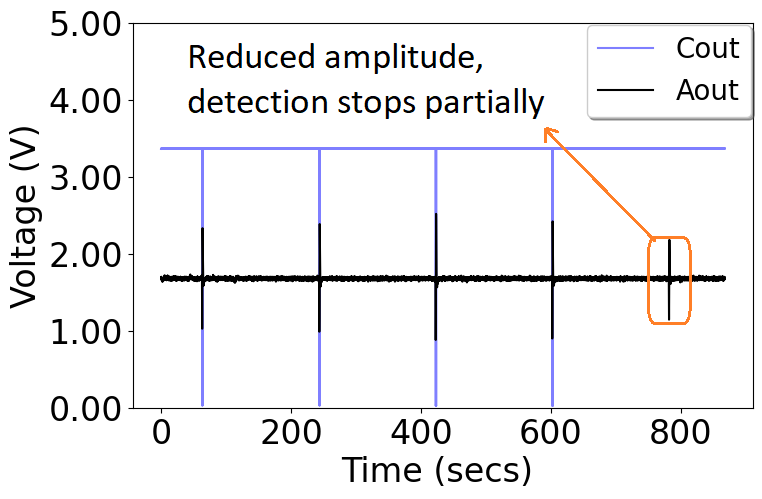
\includegraphics[width=\textwidth]{figures/gradual_degradation_dust/Stage2.png}
%		\caption{Degraded Sensor : 1/5 miss}
%		\label{fig:pir_sensor_classIII_fault_bad2_moved}
%	\end{subfigure}		
%	\hspace{1ex}
%	\begin{subfigure}[t]{0.23\textwidth}
%		\centering
%		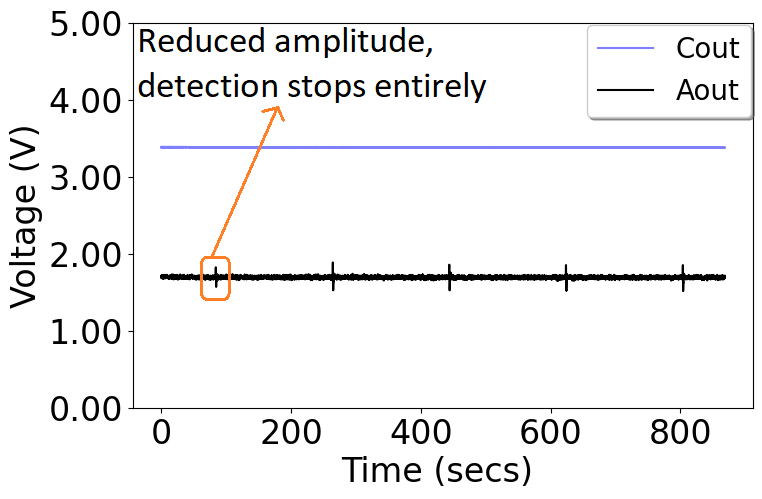
\includegraphics[width=\textwidth]{figures/gradual_degradation_dust/Stage3.png}
%		\caption{Failed Sensor : 5/5 miss}
%		\label{fig:pir_sensor_classIII_fault_bad3_moved}
%	\end{subfigure}	
%	\caption{Dust gradually building up in different degrees causing Class III faults -- \ca is a clean sensor and dust gradually builds up \cb -- \cd at which stops detecting obstacles.}
%	\label{fig:pir_sensor_classIII_fault_gradual_moved}
%\end{figure*}

%\subsubsection{Gradual Degradation in Class III faults} To study the effect of gradual failures occurring in Class III, we divided a spatula of chalk-dust (approximately one-fourth of a teaspoon) and measured the effect of the dust on the response of the sensor by incrementally adding dust at each stage and measuring performance in our controlled environment. The experiment is summarized in {\bfseries Fig.~\ref{fig:pir_sensor_classIII_fault_gradual}}.The obstacle detection process works till a reduced amplitude of \aout (Figure~\ref{fig:pir_sensor_classIII_fault_bad1}), below which the sensor begins missing some obstacle instances. This process aggravates as more dust is accumulated on the sensor until a stage when there is a complete failure (Figure~\ref{fig:pir_sensor_classIII_fault_bad3}).




%\subsection{Failures -- A Quantitative Analysis} 
%\label{subsec:quantify}
%A failure is said to impact the sensor performace if the failure results in either false detections or missed obstacles in the sensor output (\cout), compared to a working sensor. 

%To investigate the manner in which failure can affect the reliability of the PIR sensor, we investigate the output of the sensor \ie \cout. 

%As seen in Figure~\ref{fig:pir_sensor_working}, we mark as 1 a HIGH value of \cout (when there is no obstacle detected) and mark as 0 a LOW value of \cout (when there is an obstacle detected).

% \textit{Controlled Environment} In our lab setup, we take 2 PIR sensors, one which is without the fault and one which has the faulty sensor. The 2 sensors are placed in as close a proximity to one another as possible such that -- \ca the distance between the sensors are closer than the size of the obstacle, \cb the obstacle is moved in a plane such that it comes into the detection region of both the PIR sensors simultaneously. The obstacle (we used our palm in this case) across the region of interest of the PIR sensor such that it grazed the regions of detection of both the deployed sensors at the same time and trigger the same responses from both the sensors. 

%We then calculate the absolute difference ($\delta_N$) between the \cout values of the tampered sensor~\viz  \couttampered and the reference working sensor~\viz \coutworking by summing over all observations (Refer Eqn~\ref{eqn:1}). A relatively low $\delta_N$ would imply that the tampered sensor is still in acceptable condition \ie the failure is not having much impact on the operation of the sensor. On the other hand, a high value of difference implies that the failure is much serious. \textbf{Table~\ref{tbl:fault_degree}} summarizes $\delta_N$ for a few types of failures as observed over 6-hour and 12-hour runs deployed in an Elevator. We note that in our case, the lens covered failure (8 failures per hour) is more pernicious than lens having fallen off (6 failures per hour).\\

%The numbers in the column represent misclassifications ($\delta_N$)~\ie the number of false detections (both false positives and false negatives) by the faulty sensor calculated using Equation~\ref{eqn:1}. \\

% Equation working
%\begin{equation}
%    {\tikzmarknode{d}{\highlight{red}{$\delta_N$}}} = \underset{W}{\sum} \left|C_{\text{out,tampered}} - C_{\text{out, working}}\right|,
%    \label{eqn:1}
%    \begin{tikzpicture}[overlay,remember picture,>=stealth,nodes={align=left,inner ysep=1pt},<-]
%        % For "d", i.e. delta
%        \path (d.north) ++ (0,0.6em) node[anchor=south west,color=red!67] (scalep){\textbf{misclassifications}};
%        \draw [color=red!57](d.north) |- ([xshift=-0.3ex,color=red]scalep.south east);
%    \end{tikzpicture}
%\end{equation}

%\begin{equation}
%{\tikzmarknode{d}{\highlight{blue}{$\delta_N$}}} = \underset{}{\sum} 
%\left| {\tikzmarknode{t}{\highlight{red}{$C_{\text{out,tampered}}$}}} - {\tikzmarknode{w}{\highlight{green}{$C_{\text{out, working}}$}}}\right|,
%\label{eqn:1_moved}
%\begin{tikzpicture}[overlay,remember picture,>=stealth,nodes={align=left,inner ysep=1pt},<-]
%% For "d", i.e. delta
%\path (d.south) ++ (0,-0.6em) node[anchor=north west,color=blue!67] (scalep){\textbf{misclassifications}};
%\draw [color=blue!57](d.south) |- ([xshift=0.3ex,color=red]scalep.south east);
%\end{tikzpicture}
%\begin{tikzpicture}[overlay,remember picture,>=stealth,nodes={align=left,inner ysep=1pt},<-]
%% For "t", i.e. tampered
%\path (t.north) ++ (0,0.6em) node[anchor=south east,color=red!67] (scalep){\textbf{tampered}};
%\draw [color=red!57](t.north) |- ([xshift=-10ex,color=red]scalep.south east);
%\end{tikzpicture}
%\begin{tikzpicture}[overlay,remember picture,>=stealth,nodes={align=left,inner ysep=1pt},<-]
%% For "w", i.e. working
%\path (w.north) ++ (0,0.6em) node[anchor=south west,color=teal] (scalep){\textbf{working}};
%\draw [color=teal!57](w.north) |- ([xshift=-0.3ex,color=green]scalep.south east);
%\end{tikzpicture}
%\end{equation}\\
%The degree of reliability required can be tuned according to the application. 
%\ashish{need a good terminology for false positive and false negatives.}

%\textbf{Granularity of Misclassifications} 
%A tunable parameter that arises while quantifying the impact of failure is the number of samples over which the misclassification is measured. The two extremes are -- \ca comparing sample by sample between the sensor values, and \cb capturing the entire measurement duration and comparing the (average) \cout values. More generally, 

%To ease computation, we can also compute $\delta_N$ by dividing the time series into equal size chunks called \textit{windows} (W) and computing the difference between average \cout values of \tampered and \working. In long deployments, we used a window size, $W$ = 1024 samples, which comes to a window of time duration 40 seconds.

%In Table~\ref{tbl:fault_degree} we see that lens covered fault gives around 8 incorrect readings per hour compared to pyroelectric window broken scenario. We observe that obstruction due to foreign substances either on the lens or on the pyroelectric window can lead to highly erroneous sensor data.

%\noindent \textbf{Summary:} Quantifying the impact of a failure gives hints on how pernicious specific failures are \textit{once they have been detected}. We \textit{do not use Eqn~\ref{eqn:1} as a way to detect failures}. Instead, it serves as a guideline to develop a taxonomy of failures.

%\begin{table}\small
%	\centering
%	\caption{\textbf{Misclassifications} analysis for different failures.%The numbers indicate the deviation (as defined in~\ref{eqn:1} between $C_{out}$ values of a faulty sensor from that of a working sensor. 
%		Higher number indicates increased degree of failure.}
%	%\begin{tabular}{lcccc}
%	\begin{tabular}{p{1.05cm}p{1.15cm}p{1.45cm}p{1.35cm}p{1.45cm}}
%		\hline
%		\bfseries \textsc{Failure} & \bfseries \textsc{Lens Dislodged} & \bfseries \textsc{Lens Covered} & \bfseries \textsc{Heat Damage} & \bfseries \textsc{Humidity Damage}\\
%		\hline \hline
%		\rowcolor{gray!20} $\delta_N$$^1$ & 35 & 48 & 29 & 48 \\
%		$\delta_N$$^2$ & 69 & 94  & 53 & 87 \\
%		\hline 
%	\end{tabular}\\
%	\label{tbl:fault_degree_moved}
%	\vskip1pt
%	\quad \raggedright
%	$^1$ 6 hour run, $^2$ 12 hour run
%\end{table}

%Moved to main paper
%\subsection{Analyzing Failures in Time Domain}
%
%The variance of \aout during a period with no obstacle can be used to get hints on Class I faults (lens dislodged) and Class III faults (lens covered). In particular, compared to a working sensor where the lens is mounted correctly, we observe a drop in variance when the lens is covered and a rise in variance when the lens has fallen. In other words, $\sigma$(\aout)$|_{Class\ III}$ $\leq$ $\sigma$(\aout)$|_{Working}$ $\leq$ $\sigma$(\aout)$|_{Class\ I}$, where $\sigma$(\aout)$|_{X}$ denotes the variance of \aout under scenario X. We extend this to develop a preliminary fault detection algorithm that can be used to detect Class I and Class III faults. This requires the computation of two variance-based thresholds ($T_L$, $T_H$) to deduce the status of the lens. 
%However, we note that using the variance of \aout is not viable in all practical conditions. In particular, this method works only during \textit{quiet} times \ie in the absence of an obstacle which is a \textit{disadvantage}. As a result, this approach is suited for outside office or regular business hours of operation such as weekends. Therefore, we need to perform additional characterization of the \aout output signal to reason about the failures.

%\renewcommand\algorithmiccomment[1]{%
{\it /* {#1} */} %
}
\renewcommand{\algorithmicrequire}{\textbf{Input: }}
\renewcommand{\algorithmicensure}{\textbf{Output: }}
\renewcommand{\algorithmicforall}{\textbf{for each}}
\begin{algorithm}%[H]
\footnotesize
	\begin{algorithmic}[1]
	        \STATE \algorithmicrequire{Given the \aout signal, Supervised learning model $M$, window size $W$}
	        \STATE \algorithmicensure{Return if the sensor is working or faulty with the type of fault, if applicable}
            \IF {No occupancy}
                \STATE  \COMMENT{Use variance-based threshold to determine faults }
                \STATE $var \gets variance (A_{out}[1:W])$
                \IF{$var$ < $T_L$}
                    \RETURN \textsc{Fault: Lens cap is covered}
                \ELSIF{$var$ > $T_H$}
                    \RETURN \textsc{Fault: Lens cap has fallen off}
                \ELSE
                    \RETURN \textsc{Working: No lens-related fault}
                \ENDIF
            \ELSE
                \STATE \COMMENT{Transform signal to frequency domain}
                \STATE ($F_1, F_2, F_3, \ldots, F_{N})$) $\gets$ FFT\_Coeff ($A_{out}[1:W]$)
                \STATE \textsc{Fault\_type} $\gets$ M($F_1, F_2, F_3, \ldots, F_{N}$)
                \RETURN \textsc{Fault\_type}
            \ENDIF
    \end{algorithmic}
\caption{PIR Sensor Lens Fault Detection Algorithm}
\label{alg:fault_detection}
\end{algorithm}

%%%%%%%%%%%%%%%%%%%%%%%%%%%%%
% DEPLOYMENT IN CAFETERIA
%%%%%%%%%%%%%%%%%%%%%%%%%%%%%





%%%%%%%%%%%%%%%%%%%%%%%%%%%%%
% END DEPLOYMENT IN CAFETERIA
%%%%%%%%%%%%%%%%%%%%%%%%%%%%%

% A detailed study of how the sensor works and its functional block diagram gives us an insight into detecting and characterizing the faults that could result from sensor failures.



%%% TO BE UNCOMMENTED
% \begin{figure*}
% 	%\vspace{-2\baselineskip}
% 	\centering
% 	\subfloat[128 sample window \label{fig:conf_matrix_varying_window_sizes_fft_a}]{%
% 		\includegraphics[width=0.50\linewidth]{figures/pir/varying_window_sizes/FFT_Results/Weekday/FFT_RandomForest_Weekday_24hour_128.png}}
% %   \vspace{-1.2em}
% 	\subfloat[256 sample window \label{fig:conf_matrix_varying_window_sizes_fft_b}]{%
% 		\includegraphics[width=0.50\linewidth]{figures/pir/varying_window_sizes/FFT_Results/Weekday/FFT_RandomForest_Weekday_24hour_256.png}}\\
% % 	\vspace{-1.2em}
% 	\subfloat[512 sample window \label{fig:conf_matrix_varying_window_sizes_fft_c}]{%
% 		\includegraphics[width=0.50\linewidth]{figures/pir/varying_window_sizes/FFT_Results/Weekday/FFT_RandomForest_Weekday_24hour_512.png}}
% % 	\vspace{-1.2em}
% 	\subfloat[1024 sample window \label{fig:conf_matrix_varying_window_sizes_fft_d}]{%
% 		\includegraphics[width=0.50\linewidth]{figures/pir/varying_window_sizes/FFT_Results/Weekday/FFT_RandomForest_Weekday_24hour_1024.png}}
% 	\caption{\textbf{Effect of varying window sizes on the classification of faults} using FFT Coefficients (Dataset: CSL Elevator with 5 PIR sensors -- we do not have Class V fault here) -- NEED TO REASON OUT HOW FFT ON 1024 IS GIVING SUCH NUMBERS BY TRYING ON OTHER DATASETS }
% 	\label{fig:conf_matrix_varying_window_sizes_fft}
% 	\vspace{-2\baselineskip}
% \end{figure*}


%\noindent \textbf{Effect of window size on accuracy of fault detection} We emphasize that the optimal window size depends on the deployment. To get an idea, we deployed PIR sensors in 2 deployments - both of which were captured over business hours before the onset of the covid-19 pandemic
%\begin{itemize}
%    \item Cafeteria of a office building in Bangalore, India,
%    \item Elevator of a university building in Illinois, USA: 
%\end{itemize}


% \begin{table}[b]
%         %\hrulefill
%         \caption{\textbf{Effect of Window sizes} on the fault detection accuracy}
%         %\resizebox{\textwidth}{!}{
%         \begin{tabular}{p{3cm}p{1cm}p{1cm}p{1cm}p{1cm}}
%         %\begin{tabular}{p{1.25cm}p{1cm}p{1.5cm}p{1.5cm}
%             \hline
%             \bfseries \textsc{Experiment Setup} & \bfseries \textsc{6 seconds}$^1$ & \bfseries \textsc{12 seconds}$^2$ & \bfseries \textsc{24 seconds}$^3$ & \bfseries \textsc{48 seconds}$^4$\\
%             \hline \hline
%             \rowcolor{gray!20} Elevator (University Building - 24 hour weekend deployment) & 69.9\% & 74.5\%  & 77.33\% & 83.1\% \\
%              Elevator (University Building - 24 hour weekday deployment) & 46.8\% & 45.7\% & 50.5\% & 53.6\%\\
%             % \rowcolor{gray!20} Cafeteria (Office Building - Lunchtime deployment) &  &  &  & \\
%             \hline 
%         \end{tabular}\\
%         \vskip1pt 
%         \raggedright \raggedright
%         $^1$ 128-sample,
%         $^2$ 256-sample,
%         $^3$ 512-sample,
%         $^4$ 1024-sample window
%         %}
%         \label{tbl:window_effects}
%         \vspace{-1.5\baselineskip}
% \end{table}


%%% TO BE UNCOMMENTED
% \begin{figure*}
% 	%\vspace{-\baselineskip}
% 	\centering
% 	\subfloat[128 sample window \label{fig:conf_matrix_varying_window_sizes_psd_a}]{%
% 		\includegraphics[width=0.49\linewidth]{figures/pir/varying_window_sizes/PSD_Results/Weekday/PSD_FFT_Weekday_24hour_128.png}}
% %   \vspace{-1.2em}
% 	\subfloat[256 sample window \label{fig:conf_matrix_varying_window_sizes_psd_b}]{%
% 		\includegraphics[width=0.49\linewidth]{figures/pir/varying_window_sizes/PSD_Results/Weekday/PSD_FFT_Weekday_24hour_256.png}}\\
% % 	\vspace{-1.2em}
% 	\subfloat[512 sample window \label{fig:conf_matrix_varying_window_sizes_psd_c}]{%
% 		\includegraphics[width=0.49\linewidth]{figures/pir/varying_window_sizes/PSD_Results/Weekday/PSD_FFT_Weekday_24hour_512.png}}
% % 	\vspace{-1.2em}
% 	\subfloat[1024 sample window \label{fig:conf_matrix_varying_window_sizes_psd_d}]{%
% 		\includegraphics[width=0.49\linewidth]{figures/pir/varying_window_sizes/PSD_Results/Weekday/PSD_FFT_Weekday_24hour_1024.png}}
% 	\caption{\textbf{Effect of varying window sizes on the classification of faults} using peaks of the Power Spectral Density (PSD) as a feature}
% 	\label{fig:conf_matrix_varying_window_sizes_psd}
% \end{figure*}

%%% TO BE UNCOMMENTED
% \begin{table*}[hbt]
%     \centering
%     \caption{\textsc{Deployment Statistics} of Misclassifications from a 4 hr. deployment at a cafeteria in a student plaza.}
%     \label{tbl:cafeteria_deployment}
%     \begin{tabular}{ | l | m{1.00cm} | m{1.00cm} | m{1.00cm} | m{1.00cm} | m{1.00cm} | m{1.00cm} | m{1.00cm} | m{1.00cm} | m{1.00cm} | m{1.00cm} |}
%         \hline
%         \multirow{2}{*}{\bfseries Fault Class} & 
%         \multicolumn{2}{c|}{\bfseries Window = 1024} & 
%         \multicolumn{2}{c|}{\bfseries Window = 512} & 
%         \multicolumn{2}{c|}{\bfseries Window = 256} & 
%         \multicolumn{2}{c|}{\bfseries Window = 128} &
%         \multicolumn{2}{c|}{\bfseries Window = 32} \\
%         \cline{2-11}
%         \bfseries   & \bfseries $F_N$ &  \bfseries $F_P$ & 
%         \bfseries $F_N$ &  \bfseries $F_P$  &
%         \bfseries $F_N$ &  \bfseries $F_P$ &
%         \bfseries $F_N$ &  \bfseries $F_P$ &
%         \bfseries $F_N$ &  \bfseries $F_P$ \\ \hline \hline
%             Class I &  27 & 0  & 54 & 0 & 111 & 0 & 215 & 0 & 1050 & 9 \\ \hline
%             Class II &  35 & 0  & 68 & 0 & 163 & 0 & 353 & 0 & 1834 & 12 \\ \hline
%             Class III &  26 &  0 & 50 & 0 & 95 & 0 & 178 & 0 & 771 & 14\\ \hline
%             Class IV &  0 & 0  & 0 & 0 & 0 & 0 & 0 & 0 & 68 & 17\\ \hline
%             Class V & 226 & 0 & 452 & 0 & 905 & 0 & 1811 & 0 & 7246 & 0\\ \hline
%     \end{tabular}
% \end{table*}


%\section{Warm-Up Behavior Analysis} PIR sensors have a period of \textit{warm-up} period of around 30 seconds, which is a manufacturer provided time, only after which the sensor is ready to detect obstacles. The warm-up time is used by the PIR sensor to calibrate itself to its surroundings. There are 2 types of warm-up behavior -- \ca Smooth warm-up and \cb Trigger warm-up.
%
%\section{Electrocardiogram (ECG) Analysis} ECG is a graph of the electrical activity of the heart. The waveform is a plot of voltage vs time and is measured using electrodes placed under the skin. each cardiac cycle also known as a heartbeat produces contraction and expansion of cardiac muscle which is represented by a certain pattern of voltage waveform, also called a normal ECG pattern. Changes in the pattern are brought about by cardiac abnormalities~\eg cardiac rhythm disturbances.
%
%There are 3 main components of a ECG waveform-- \ca P-wave which represents the depolarization of the atria, \cb QRS complex, which represents the depolarization of the ventricles and T-wave, which repolarization of ventricles.




